%----------------------------------------------------------------------------------------------------
\section{Analysis of Coulomb-nuclear interference region}
\label{sec:cni}

\> key elements of phenomenology/theory of Coulomb-nuclear interference
\>> Coulomb amplitude: ``well'' known
\>> interference formula: SWY (traditionally used) or KL (theoretically more appropriate)
\>> modulus of nuclear amplitude -- strongly constrained by data $\Rightarrow$ exponential parametrisation $\d\sigma / \d t \propto \exp( -B(t) )$; reasonable degrees of the $B(t)$ polynomial are $N_b = 1, 2, 3$ (describes well the data and many phenomenological models); $N_b = 1$ gently disfavoured by the data; fit amplitude anchored to $90\un{m}$ data at $|t| > 0.2\un{GeV^2}$
\>> phase of nuclear amplitude -- weak guidance from data $\Rightarrow$ need assumption: constant, central, peripheral (the last two as from \cite{kl94})

\> with the presented data not possible to distinguish between different models/assumptions above $\Rightarrow$ {\bf conditional} determination of parameters of interest
\>> $\rho$
\>> total cross-section and $B$ with Coulomb separated


\> interference formulae:
\>> with SWY: only constant phase and $N_b = 1$ -- only to show what would happen if the traditional approach was used
\>> with KL: nuclear phase constant/central/peripheral, $N_b = 1, 2, 3$ (exclude 1 ??)

\> nuclear phase choices -- several theoretical alternatives
\>> constant: the simplest
\>> central: need reference!
\>> peripheral -- central values and uncertainties -- need reference!


\> generalised $\chi^2$ fits (covariance matrix contained all relevant contributions: statistical, normalisation and misalignment), fits driven by Minuit

\> extensive MC tests (input: phenomenological models as well as data fits)
\>> check for bias: only small
\>> understanding/evaluation of the method response to statistical and systematic uncertainties

\> results ($\rho$, $\sigma_{\rm tot}$, $B^{\rm N}(0)$, ...)
\>> for the model choices above -- keeping phase parameters fixed at their central values from Vojt\v ech
\>> for peripheral-phase parameters being varied within their uncertainties $\Rightarrow$ uncertainty band

\> question: do we want to present a single-value result for $\rho$ (combined from fits under different models) ??

\> discuss the new value of $\sigma_{\rm tot}$ in comparison to our previous measurement \cite{prl111}; values compatible; remind in what is the new measurement better ??

\> reference to Fig.~\ref{fig:rho_s}

\begin{figure*}
\begin{center}
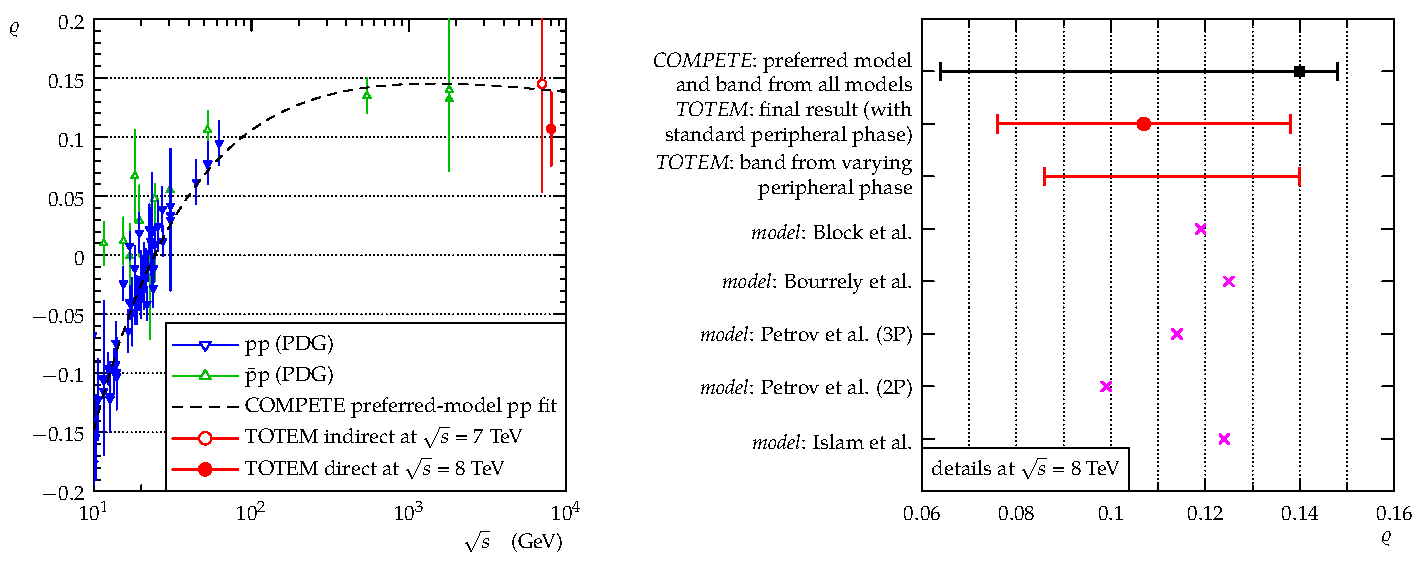
\includegraphics[width=16cm]{fig/rho_s.pdf}
\vskip-3mm
\caption{$\rho$ as a function of $s$.}
\label{fig:rho_s}
\end{center}
\end{figure*}

\> figure for $\sigma_{\rm tot}$ result ?? 
